\chapter{Conclusion and future work}
\label{CAFW}

\section{Conclusion}
\label{Conclusion}

\section{Future Work}
\label{Future Work}
Next steps would be to give the model to the lab technicians running lab experiments so that they can verify the results as seen in the output by comparing the lab results with the model output. 
With the lab results, the model can be adapted to better fit the lab results. 
This can be done by changing parameter values, or by changing the model equation. 
The user can decide to add the Monod microbial growth model to the growth of the bacteria, or adapt the Monod equation to being dependent on multiple sources. 
Using the model, the technicians can improve and validate their methods. 
If the empirical results significantly deviate from the model results, the technician can review to see if their method is good. 
They might have accidentally not added enough resources, or accidentally miscalculated the initial concentration of bacteria. 

\subsection{Other Models}
\textit{“All models are wrong, but some are useful“} — George E. P. Box \newline \newline
Each model has its pros and cons. 
Take the exponential population growth model 
\begin{align}
    \frac{dP}{dt} &= rP \\
    P(t) &= P_0e^{rt} 
\end{align}
where $P(t)$ is the population at time $t$, $P_0$ is the initial population, and $r$ is the growth rate. 
This model acts as a nice introduction to population modelling. It can accurately fit the exponential growth bacteria experience in a petri dish. 
However, this basic model does not account for a spatial and resource consumption. 
Eventually the bacteria run out of space and resources, and start to die out. 
A population can not grow exponentially forever, the resources can only support a maximum population, the carrying capacity. 
The model can be adapted to include a carrying capacity (the max population level that can be reached), where the new updated model is 
\begin{align}
    \frac{dP}{dt} &= rP(1-\frac{P}{K}) \\ 
    P &= \frac{K}{1 + (\frac{K-N_0}{N_0})e^{-rt}}
\end{align}
where $K$ is the carrying capacity. This adapted model, the logistic growth model better accounts for the eventual restriction of population growth. 
\newline
\Cref{fig:created:exponential_vs_logistic_growth} shows how the carrying capacity has a large influence on the speed and growth trajectory of a population. 
The logistic curve initially follows the exponential curve before the maximum growth rate is reached and starts to slow down and taper off as the population asymptotically approaches the carrying capacity $K=200$. 

A further step would be to introduce competition between other bacteria. 
For example, a $p_{0, 1}\cdot P_0 \cdot P_1$ term can be subtracted from the logistic growth curve. 
This term accounts for competition between Populace 0 and Populace 1, with $p_{0, 1}$ being the interaction factor between $P_0$ and $P_1$. 
Assuming $P_0$ is being looked at and $P_0$ has a high value, if $P_1$ is high, then a lot of $P_0$ is going to die out due to the competition with $P_1$. 
If $P_1$ has a low population, then not many $P_0$ are going to die out due to less competition with $P_1$. \\ 

The model can be further extended by accounting for temperature, pH, more interactions between other agents, the constant addition and removal of other agents, and other considerations. 

\subsubsection{Spatial simulations}
https://www.sciencedirect.com/science/article/abs/pii/S0022519318305368
The ODE models work very nicely when there is no consideration for space and 2D/3D-space dimensionality. 
Spatial models complicate the simulation, making it harder to analyze. 
Data collection and analysis becomes harder. 
Unique and novel analysis and visualization methods have to be created to be able to represent and visualize the data through space and time. 
\paragraph{PDE}
PDE are the next logical step to add space to an ODE model. The general formula, as given by 
\[
    \frac{\partial u}{\partial t} = D\nabla^2u + f(u, x, y, \dots, t)
\] where $u(x, y, \dots, t)$ is the population density of interest, $D$ is the diffusion constant, $\nabla^2$ is the derivative of each spatial direction, and $f(x, y, \dots, t)$ is the function encapsulating growth, death, and interactions dynamics. 
\subparagraph{Discretization}
The dimensions can be discretized into boxes of dimensions $\delta x, \delta y, \dots$. 
This transforms the PDE into a system of difference equations, which can be solved numerically. 
For example, the Laplacian term $\nabla^2 u$ in 2D can be approximated using finite differences as:
\[
    \nabla^2 u \approx \frac{u_{i+1,j} - 2u_{i,j} + u_{i-1,j}}{\delta x^2} + \frac{u_{i,j+1} - 2u_{i,j} + u_{i,j-1}}{\delta y^2}
\]
where $u_{i,j}$ represents the value of $u$ at the grid point $(i, j)$. 
This discretization allows the PDE to be solved iteratively over a grid, enabling spatial simulations of population dynamics. 
Each box can be represented by a matrix, and the population value can be displayed as a heatmap using visualization software. 


\begin{figure}
    \centering
    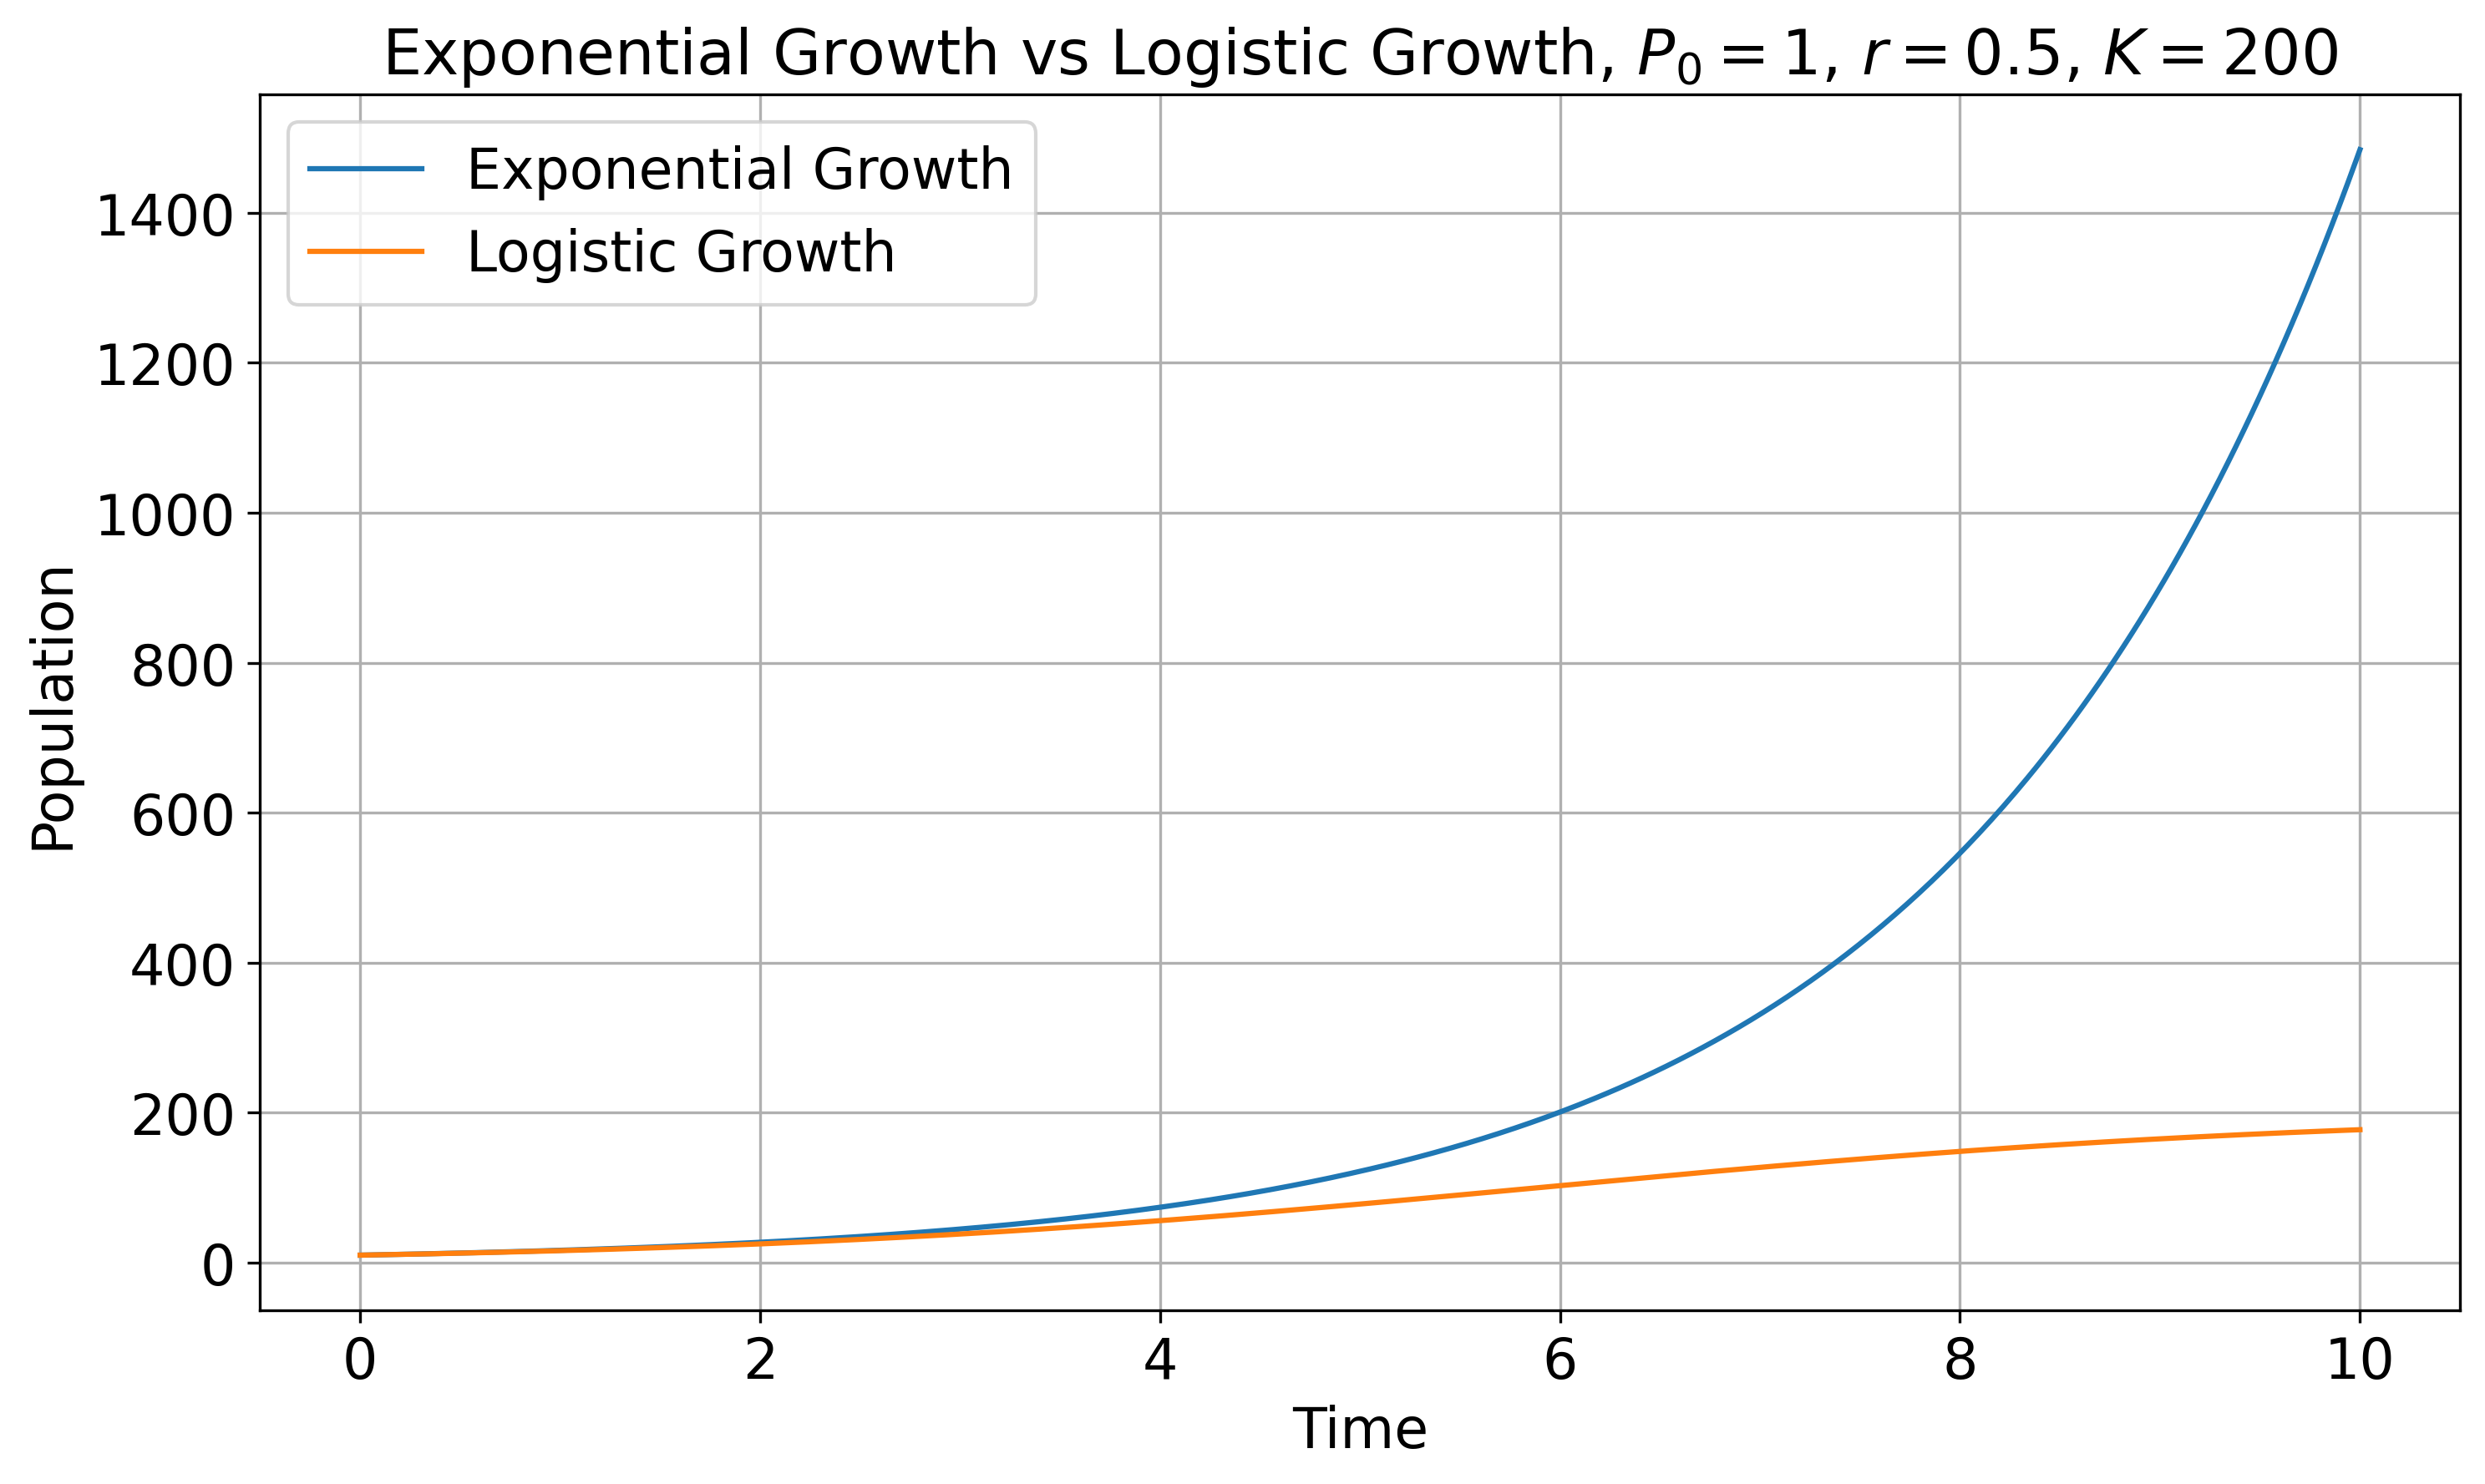
\includegraphics[width=0.5\linewidth]{Plots/Created/exponential_vs_logistic_growth.png}
    \caption{Exponential growth curve vs logistic growth}
    \label{fig:created:exponential_vs_logistic_growth}
\end{figure}